% >8-----------------------------------------------------------------------------------------------------------------8<

\chapter{Resolução do Problema Estacionário}
\section{Definição da Formulação Forte}

  Dada uma função $f : [0,1] \to \mathbb{R}$ e constantes $\alpha > 0$, $\beta \geq 0$ e $\gamma \geq 0$, queremos encontrar a função $u : [0,1] \to \mathbb{R}$ tal que:

  \begin{center}
    $(S) = \begin{cases}
      -\alpha u_{xx}(x) + \beta u(x) + \gamma u_{x}(x) = f(x) \\
      \\
      u(0) = u(1) = 0
    \end{cases}$
  \end{center}

  Sendo $(S)$ conhecido como a formulação forte do problema.

\section{Transição da Formulação Fraca para o Problema Aproximado}

  Nesse momento iremos realizar uma série de manipulações algébricas para deixar a primeira equação em um formato mais próximo de uma formulação fraca, que é mais adequada para análise teórica e para implementação numérica.

Visto que $-\alpha u_{xx}(x) + \beta u(x) + \gamma u_{x}(x) = f(x)$

Podemos multiplicar ambos os lados por uma função $v(x)$ tal que $v(1) = v(0) = 0$ que nos ajude a eliminar a segunda derivada $u_{xx}$:

\begin{align*}
  -\alpha u_{xx}(x) + \beta u(x) + \gamma u_{x}(x) &= f(x) \\
  \Big[-\alpha u_{xx}(x) + \beta u(x) + \gamma u_{x}(x)\Big]v(x) &= f(x)v(x)\\
  -\alpha u_{xx}(x)v(x) + \beta u(x)v(x) + \gamma u_{x}(x)v(x) &= f(x)v(x)\\
  \int^{1}_{0} \Big[-\alpha u_{xx}(x)v(x) + \beta u(x)v(x) + \gamma u_{x}(x)v(x)\Big] dx &= \int^{1}_{0} f(x)v(x) dx\\
  \int^{1}_{0} -\alpha u_{xx}(x)v(x) dx + \int^{1}_{0} \beta u(x)v(x) dx + \int^{1}_{0} \gamma u_{x}(x)v(x) dx &= \int^{1}_{0} f(x)v(x) dx
\end{align*}

Sabemos que dadas funções $f$ e $g$:

\begin{align*}
  \int f(x)g'(x)dx &= f(x)g(x) - \int f'(x)g(x)dx
\end{align*}

Logo, realizando a integração por partes no primeiro termo na equação:

\begin{align*}
    \int^{1}_{0} f(x)v(x) dx &= -\alpha \Big[u_{x}(x)v(x) \bigg|^{1}_{0} - \int^{1}_{0} u_{x}(x)v_{x}(x) dx\Big] + \int^{1}_{0} \beta u(x)v(x) dx + \int^{1}_{0} \gamma u_{x}(x)v(x) dx \\
    \int^{1}_{0} f(x)v(x) dx &= -\alpha \Big[(u_{x}(1)v(1) - u_{x}(0)v(0)) - \int^{1}_{0} u_{x}(x)v_{x}(x) dx\Big] + \int^{1}_{0} \beta u(x)v(x) dx + \int^{1}_{0} \gamma u_{x}(x)v(x) dx \\
    \int^{1}_{0} f(x)v(x) dx &= -\alpha \Big[\cancel{(u_{x}(1)v(1) - u_{x}(0)v(0))} - \int^{1}_{0} u_{x}(x)v_{x}(x) dx\Big] + \int^{1}_{0} \beta u(x)v(x) dx + \int^{1}_{0} \gamma u_{x}(x)v(x) dx  \\
    \int^{1}_{0} f(x)v(x) dx &= \alpha \int^{1}_{0} u_{x}(x)v_{x}(x) dx + \beta \int^{1}_{0} u(x)v(x) dx + \gamma \int^{1}_{0} u_{x}(x)v(x) dx \\
\end{align*}

\section{Definição da Formulação Fraca}

  \textbf{Definição}: Pelo restante do documento, considere que uma função $g$ é ``suficientemente suave'' se ela respeitar:
  \begin{itemize}
    \item $g$ é contínua em todo o domínio;
    \item $g$ possui derivadas contínuas até a ordem necessária.
  \end{itemize}

  Seja $H$ um espaço de funções formado por funções $u$ suficientemente suaves que satisfazem $(W)$ e as condições de contorno $u(0) = u(1) = 0$. Seja $V$ um espaço das funções de teste, composto por funções $v$ suficientemente suaves e que satisfazem as condições de contorno $v(0) = v(1) = 0$.

  Dados $\alpha > 0$, $\beta \geq 0$, $\gamma \geq 0$ e uma função $f : [0,1] \to \mathbb{R}$, precisamos determinar $u : [0,1] \to \mathbb{R}$, $u \in H$, tal que, $\forall v \in V$:

  \begin{center}
    $(W) = \begin{cases}
      \displaystyle\alpha \int^{1}_{0} u_{x}(x)v_{x}(x) dx + \beta \int^{1}_{0} u(x)v(x) dx + \gamma \int^{1}_{0} u_{x}(x)v(x) dx = \int^{1}_{0} f(x)v(x) dx \\
      \\
      u(0) = u(1) = 0
    \end{cases}$
  \end{center}

\section{Definição do Problema Aproximado pelo Método de Galerkin}

O método de Galerkin consiste em aproximar o espaço das soluções por um subespaço de dimensão ?nita para encontrarmos uma solução aproximada que satisfaça a formulação fraca do problema dentro de um subespaço apropriado, permitindo a construção de uma solução computacionalmente viável. Sendo assim:

Seja $H^h$ um espaço de funções finito-dimensional composto por funções $u^h$ suficientemente suaves que satisfazem $(A)$ e as condições de contorno $u^h(0) = u^h(1) = 0$. Analogamente, seja $V^h$ um espaço de funções finito-dimensional das funções de teste, formado por funções $v^h$ suficientemente suaves que também atendem às condições de contorno $v^h(0) = v^h(1) = 0$.

Dada uma função $f : [0,1] \to \mathbb{R}$ e constantes $\alpha > 0$, $\beta \geq 0$ e $\gamma \geq 0$, queremos determinar $u^h \in H^h$ tal que, $\forall v^h \in V^h$:

\begin{center}
  $ (A) = \begin{cases}
    \displaystyle\int^{1}_{0} f(x)v^{h}(x) dx = \alpha \int^{1}_{0} u^{h}_{x}(x)v^{h}_{x}(x) dx + \beta \int^{1}_{0} u^{h}(x)v^{h}(x) dx + \gamma \int^{1}_{0} u^{h}_{x}(x)v^{h}(x) dx \\
    \\
    u^h(0) = u^h(1) = 0
  \end{cases}$
\end{center}

\section{Transição do Problema Aproximado para a Forma Matriz-vetor}

  Visto que $u^h \in H^h$, podemos tomar $u^h$ como combinação linear das funções da base de $H^h$

  Seja \[u^h(x) = \sum_{j=1}^{m} \varphi_j(x) c_j \quad\text{ e }\quad u_{x}^h(x) = \sum_{j=1}^{m} \varphi_{xj}(x)c_j\]

  Substituindo ambos na equação:

  \begin{align*}
    \alpha \int_{0}^{1} \sum_{j=1}^{m} \varphi_{xj}(x) c_j v^h_x(x)dx + \beta \int_{0}^{1} \sum_{j=1}^{m} \varphi_j(x)c_j v^h(x)dx + \gamma \int_{0}^{1} \sum_{j=1}^{m} \varphi_{xj}(x)c_j v^h(x)dx &= \int_{0}^{1} f(x) v^h(x)dx\\
    \sum_{j=1}^{m} \Big[ \alpha \int_{0}^{1} \varphi_{xj}(x) c_j v^h_x(x)dx + \beta \int_{0}^{1} \varphi_j(x)c_j v^h(x)dx + \gamma \int_{0}^{1} \varphi_{xj}(x)c_j v^h(x)dx \Big] &= \int_{0}^{1} f(x) v^h(x)dx
  \end{align*}

  Veja que podemos tomar $v^h(x)$ como sendo qualquer função da base de $V^h$.

  Logo, $\forall i \in \{1,\dots,m\}$, $v^h(x) = \varphi_i(x)$ e $v_x^h = \varphi_{xi}(x)$. Substituindo na equação:

  \begin{align*}
    \sum_{j=1}^{m} \Big[\alpha \int_{0}^{1} \varphi_{xj}(x) c_j \varphi_{xi}(x) dx + \beta \int_{0}^{1} \varphi_j(x)c_j \varphi_i(x)dx + \gamma \int_{0}^{1} \varphi_{xj}(x)c_j \varphi_i(x)dx &= \int_{0}^{1} f(x) \varphi_i(x)dx\Big] \\
    \sum_{j=1}^{m} c_j\Big[\alpha \int_{0}^{1} \varphi_{xj}(x) \varphi_{xi}(x) dx + \beta \int_{0}^{1} \varphi_j(x) \varphi_i(x)dx + \gamma \int_{0}^{1} \varphi_{xj}(x) \varphi_i(x)dx &= \int_{0}^{1} f(x) \varphi_i(x)dx \Big]
  \end{align*}

  Veja que essa equação vale $\forall i \in \{1,\dots,m\}$, dessa forma, podemos expressar o problema na forma matriz-vetor:

  $\begin{cases}
    \displaystyle\sum_{j=1}^{m} c_j \Big[ \alpha \int_{0}^{1} \varphi_{xj}(x) \varphi_{x1}(x) dx + \beta \int_{0}^{1} \varphi_j(x) \varphi_1(x)dx + \gamma \int_{0}^{1} \varphi_{xj}(x) \varphi_1(x)dx &= \int_{0}^{1} f(x) \varphi_1(x)dx \Big] \\
    \vdots \\
    \displaystyle\sum_{j=1}^{m} c_j \Big[ \alpha \int_{0}^{1} \varphi_{xj}(x) \varphi_{xi}(x) dx + \beta \int_{0}^{1} \varphi_j(x) \varphi_i(x)dx + \gamma \int_{0}^{1} d\varphi_{xj}(x) \varphi_i(x)dx &= \int_{0}^{1} f(x) \varphi_i(x)dx \Big] \\
    \vdots \\
    \displaystyle\sum_{j=1}^{m} c_j \Big[ \alpha \int_{0}^{1} \varphi_{xj}(x) \varphi_{xm}(x) dx + \beta \int_{0}^{1} \varphi_j(x) \varphi_m(x)dx + \gamma \int_{0}^{1} \varphi_{xj}(x) \varphi_m(x)dx &= \int_{0}^{1} f(x) \varphi_m(x)dx \Big]
  \end{cases}$

\section{Definição do Problema na Forma Matriz-Vetor}

  Dado uma matriz $K$ e um vetor $F$, queremos determinar $C$ tal que:

  \[(M) = \begin{cases} \mathcal{K}\mathcal{C} = \mathcal{F} \end{cases}\]

  \[
  \begin{bmatrix}
    K_{1,1} & ... & K_{1,j} & ... & K_{1,m} \\
    \vdots & \ddots & \vdots & \ddots & \vdots \\
    K_{i,1} & ... & K_{i,j} & ... & K_{i,m} \\
    \vdots & \ddots & \vdots & \ddots & \vdots \\
    K_{m,1} & ... & K_{m,j} & ... & K_{m,m}
  \end{bmatrix}
  \begin{bmatrix}
    C_1 \\ \vdots \\ C_i \\ \vdots \\ C_m
  \end{bmatrix}
  =
  \begin{bmatrix}
  F_1 \\ \vdots \\ F_i \\ \vdots \\ F_m
  \end{bmatrix}
  \]

  $\forall i, j \in \{1,\dots,m\}$ tais que $i$ e $j$ correspondam aos índices da matriz e $i$ corresponda ao índice do vetor $F$, sejam:

  \begin{align*}
  K_{i,j} &= \alpha \int_{0}^{1} \dfrac{d\varphi_i(x)}{dx} \dfrac{d\varphi_j(x)}{dx}dx + \beta \int_{0}^{1} \varphi_i(x) \varphi_j(x)dx + \gamma \int_{0}^{1} \varphi_i(x) \dfrac{d\varphi_j(x)}{dx}dx \\
  F_i &= \int_{0}^{1} f(x) \varphi_i(x) dx
  \end{align*}

\section{Definindo uma Função Base}

  Seja $x_1, \dots, x_m$ uma discretização do intervalo $[0, 1]$ tal que $\forall i \in {1, \dots, m}$, $x_{i+1} - x_i = h$. Além disso, considere $x_0 = 0$ e $x_{m+1} = 1$ como sendo os extremos do intervalo tal que $x_{m+1} - x_m = h$ e $x_1 - x_0 = h$.

  Definiremos $\varphi_i(x)$ como:

  \[\varphi_i(x) = \begin{cases}
    \dfrac{x - x_{i-1}}{h}, &\forall x \in [x_{i-1}, x_i] \\
    \dfrac{x_{i+1} - x}{h}, &\forall x \in [x_{i}, x_{i+1}] \\
    0 , &\forall x \notin [x_{i-1}, x_{i+1}]
  \end{cases}\]

  Observe que a função base $\varphi_i(x)$ é de?nida como uma função linear por partes intencionalmente de forma que a sua integração e derivação sejam simples. Além disso, $\varphi_i(x)$ é projetada para ser zero fora do intervalo $[x_{i-1}, x_{i+1}]$, o que significa que cada função base afeta apenas dois ou três pontos consecutivos. Essa escolha reduz significativamente a complexidade do sistema linear, já que a matriz resultante terá muitas entradas nulas. Isso nos é benéfico pois então trabalharemos com matrizes esparsas, que são computacionalmente mais eficientes, tanto em termos de armazenamento quanto de tempo de processamento.

  Perceba também que:

  \[\varphi_i(x_i) = \dfrac{x_i - x_{i-1}}{h} = \dfrac{h}{h} = 1\]

\chapter{Cálculo das Locais}

\section{Matriz Local}

  Observe que, pela definição de $\varphi_i(x)$, $K_{i,j} = 0$ quando $|i-j| < 2$ Logo, podemos limitar nossa o intervalo de integração visto que restante do intervalo resultará sempre em zero. Faremos no cálculo das matrizes $K^e_{ij}$ locais de cada elemento e utilizando a notação local para as funções da base.

  \begin{align*}
  K^{e}_{i,j} &= \alpha \int_{x^{e-1}}^{x^e} \varphi_{xi}(x) \varphi_{xj}(x) dx + \beta \int_{x^{e-1}}^{x^e} \varphi_i(x) \varphi_j(x)dx + \gamma \int_{x^{e-1}}^{x^e} \varphi_i(x) \varphi_{xj}(x) dx \\
  K^{e}_{a,b} &= \alpha \int_{x_1^{e-1}}^{x_2^e} \varphi_{xa}^e(x) \varphi_{xb}^e(x)dx + \beta \int_{x_1^{e-1}}^{x_2^e} \varphi_a^e(x) \varphi_b^e(x)dx + \gamma \int_{x_1^{e-1}}^{x_2^e} \varphi_a^e(x) \varphi_{xb}^e(x)dx
  \end{align*}

  Para podermos utilizar a quadratura gaussiana como técnica de integração, precisaremos modificar nosso intervalo de $[0,1]$ para $[-1,1]$ visto que essa é a condição para o uso dessa técnica.

  Seja $x(\xi, e)$ a função que converte de $\xi$ para $x$ tal que $x(\xi, e) = \dfrac{h}{2}(\xi + 1) + x_{e-1}$.

  \[\text{Seja }\quad\phi_n(\xi) = \begin{cases}
    \dfrac{1 - \xi}{2}\quad&\text{, se } n = 1 \\[10pt]
    \dfrac{1 + \xi}{2}\quad&\text{, se } n = 2 \\
  \end{cases}\quad\text{ e seja }\quad\dfrac{d\phi_n}{d\xi}(\xi) = \begin{cases}
    \dfrac{-1}{2}\quad&\text{, se } n = 1 \\[10pt]
    \dfrac{1}{2}\quad&\text{, se } n = 2 \\
  \end{cases}\]

  tal que: \[\phi_n(\xi) = \varphi_n^{e}(x(\xi, e))\]

  \begin{align*}
    K^{e}_{a,b} &= \alpha \int_{-1}^{1} \varphi_{xa}^e(x(\xi, e)) \varphi_{xb}^e(x(\xi, e)) \dfrac{h}{2}d\xi + \beta \int_{-1}^{1} \varphi_a^e(x(\xi, e)) \varphi_b^e(x(\xi, e))\dfrac{h}{2}d\xi \\
    &+ \gamma \int_{-1}^{1} \varphi_a^e(x(\xi, e)) \varphi_{xb}^e(x(\xi, e))\dfrac{h}{2}d\xi \\
  \end{align*}

  Como, por definição, $\phi_n(\xi) = \varphi_n^{e}(x(\xi, e))$, então:

  \begin{align*}
    K^{e}_{a,b} &= \alpha \int_{-1}^{1} \phi_{\xi a}(\xi) d\phi_{\xi b}(\xi)\dfrac{h}{2}\dfrac{2}{h}\dfrac{2}{h}d\xi + \beta \int_{-1}^{1} \phi_a(\xi) \phi_b(\xi)\dfrac{h}{2}d\xi + \gamma \int_{-1}^{1} \phi_a(\xi) \phi_{\xi b}(\xi) \dfrac{h}{2}\dfrac{2}{h}d\xi \\
    K^{e}_{a,b} &= \alpha \int_{-1}^{1} \phi_{\xi a}(\xi) \phi_{\xi b}(\xi)\dfrac{2}{h}d\xi + \beta \int_{-1}^{1} \phi_a(\xi) \phi_b(\xi)\dfrac{h}{2}d\xi + \gamma \int_{-1}^{1} \phi_a(\xi) \phi_{\xi b}(\xi)d\xi \\
    K^{e}_{a,b} &= \dfrac{2\alpha}{h} \int_{-1}^{1} d\phi_{\xi a}(\xi) \phi_{\xi b}(\xi)d\xi + \dfrac{\beta h}{2} \int_{-1}^{1} \phi_a(\xi) \phi_b(\xi)d\xi + \gamma \int_{-1}^{1} \phi_a(\xi) \phi_{\xi b}(\xi)d\xi
  \end{align*}

\section{Vetor Local}

  Assim como fizemos com $K^e_{i,j}$, podemos fazemos o mesmo com a $F_i^e$ local de cada elemento.

  \begin{align*}
    F_a^e &= \int_{0}^{1} f(x) \varphi_i(x) dx \\
    F_a^e &= \int_{x_1^e}^{x_2^e} f(x) \varphi_a^e(x) dx \\
    F_a^e &= \int_{-1}^{1} f(x(\xi, e)) \varphi_a^e(x(\xi, e))\dfrac{h}{2} d\xi \\
    F_a^e &= \dfrac{h}{2} \int_{-1}^{1} f(x(\xi, e)) \phi_a(\xi) d\xi
  \end{align*}

  Visto que sabemos montar a matriz $K$ a partir de $K^e_{a,b}$ e o vetor $F$ a partir de $F_a^e$, os coeficientes do vetor $C$ podem finalmente ser calculados.

\chapter{Alguns dos Testes Realizados}

  Para testarmos o procedimento, precisamos primeiro escolher uma função $u(x)$ que satisfaça $u(0) = u(1) = 0$. Também precisamos definir valores para $\alpha$, $\beta$ e $\gamma$. Nesse caso em específico, selecionamos valores arbitrários somente para testes:

  \begin{code}
  alpha = 1                               # constant value
  beta = 1                                # constant value
  gamma = 1                               # constant value
  u = (x) -> sin(pi * x)
  \end{code}

  Em seguida, podemos calcular o valor esperado para a função $f(x)$ para que possamos calcular o erro do nosso método. $f(x)$ precisa necessariamente satisfazer:

  \[f(x) = -\alpha u_{xx}(x) + \beta u(x) + \gamma u_{x}(x)\]

  Sendo assim:

  \begin{align*}
    f(x) &= -\alpha u_{xx}(x) + \beta u(x) + \gamma u_{x}(x) \\
    f(x) &= -\alpha (\sin(\pi x))_{xx} + \beta \sin(\pi x) + \gamma (\sin(\pi x))_{x} \\
    f(x) &= -\alpha (\pi \cos(\pi x))_{x} + \beta \sin(\pi x) + \gamma \pi \cos(\pi x) \\
    f(x) &= -\alpha \pi^2 (- \sin(\pi x)) + \beta \sin(\pi x) + \gamma \pi \cos(\pi x) \\
    f(x) &= \alpha \pi^2 \sin(\pi x) + \beta \sin(\pi x) + \gamma \pi \cos(\pi x) \\
  \end{align*}

  Logo:

  \begin{code}
  f = (x) -> alpha*pi^2 * sin(pi*x) + beta*sin(pi*x) + gamma*pi*cos(pi*x)
  \end{code}

  Sendo assim, ao rodarmos como código com o número de elementos variando de $1$ até $131071$ ($2^1 - 1$ até $2^{17} - 1$), obtemos os seguintes gráficos:

  \begin{figure}[H]
    \centering
    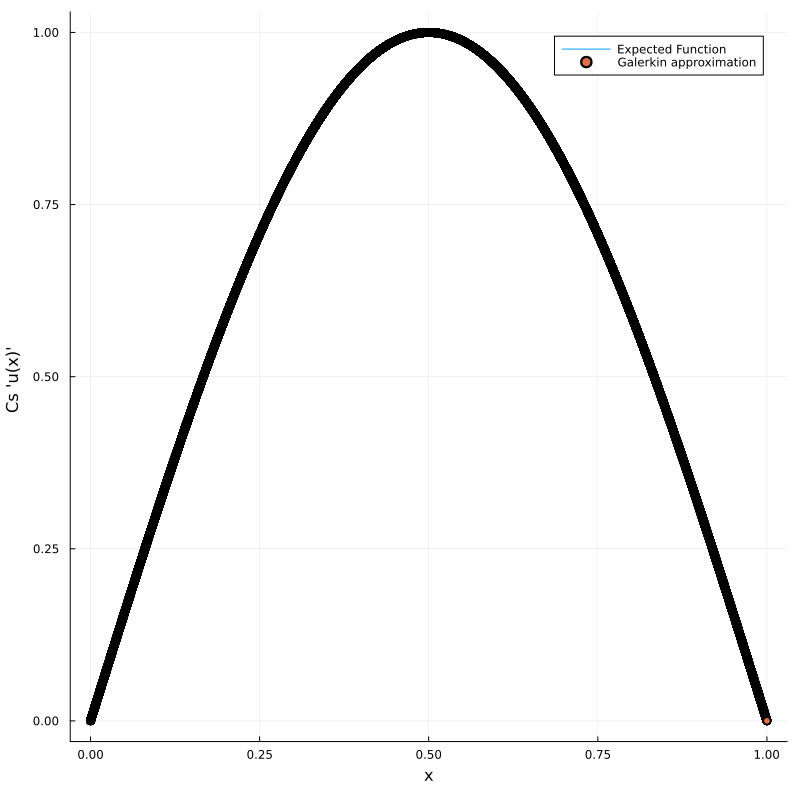
\includegraphics[width=0.45\linewidth]{Galerkin-generic-ode-error-graph.png}
    \caption{Gráfico que mostra a função original e nossos pontos aproximados por cima (Não é possível ver ambos muito bem pois o número de pontos está bem alto).}
  \end{figure}

  \begin{figure}[H]
    \centering
    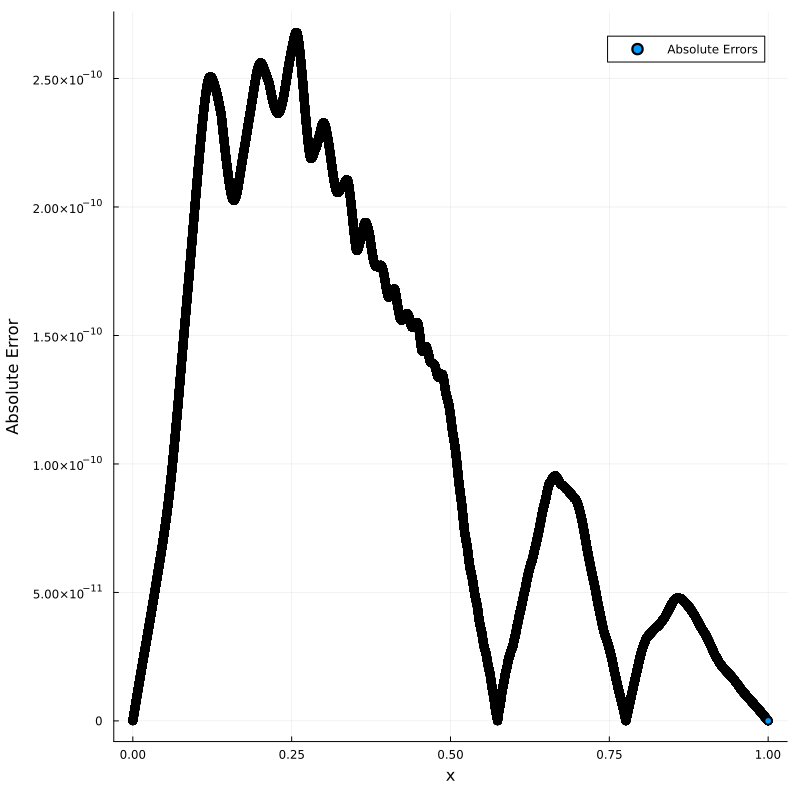
\includegraphics[width=0.45\linewidth]{Galerkin-generic-ode-absolute-errors-graph.png}
    \caption{Gráfico que mostra a distância no eixo $y$ para cada ponto encontrado pelo nosso método em comparação com a função original.}
  \end{figure}

  \begin{figure}[H]
    \centering
    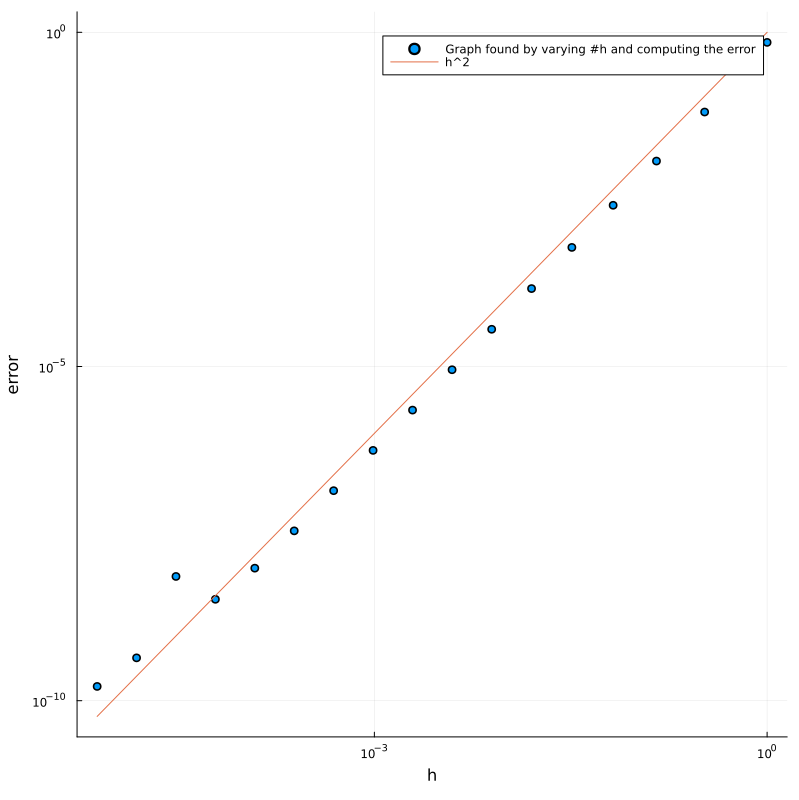
\includegraphics[width=0.5\linewidth]{Galerkin-generic-ode-errors.png}
    \caption{Gráfico que mostra os erros conforme o espaçamento entre cada elemento varia.}
  \end{figure}

  Veja que o gráfico da convergência do erro apresenta inclinação $2$ na escala logarítmica, o que significa que o erro está na ordem de $h^2$, que é o esperado.


% >8-----------------------------------------------------------------------------------------------------------------8<